\documentclass[11pt, oneside]{article}   	% use "amsart" instead of "article" for AMSLaTeX format
\usepackage{geometry}                		% See geometry.pdf to learn the layout options. There are lots.
\geometry{letterpaper}                   		% ... or a4paper or a5paper or ... 
%\geometry{landscape}                		% Activate for for rotated page geometry
%\usepackage[parfill]{parskip}    		% Activate to begin paragraphs with an empty line rather than an indent
\usepackage{graphicx}				% Use pdf, png, jpg, or eps� with pdflatex; use eps in DVI mode
								% TeX will automatically convert eps --> pdf in pdflatex		
\usepackage{amssymb}
\usepackage{fancyref,multicol,fixltx2e}

\title{A Microfluidic Device for Measuring Aerotaxis}
\author{Kiarash Adl, Brian Djaja, Katarina Struckmann and Logan Williams}
%\date{}							% Activate to display a given date or no date

\begin{document}
\maketitle
%\section{}
%\subsection{}
\section{Abstract}

Bacteria rely heavily on sensing environmental gradients to survive and reproduce. While significant effort has been made to understand responses to chemical gradients, or chemotactic responses, less literature exists characterizing responses to gas gradients, or aerotactic responses. This study employed a three-channel microfluidic device fabricated from PDMS to characterize aerotactic bacterial motion. In the presence of a gradient of nitrogen and oxygen, movement of the organism \textit{B. subtilis} tended toward oxygen and away from nitrogen, demonstrating an aerotactic response.

\section{Introduction}

The movement of bacteria in response to a gas gradient, aerotaxis, is a field that has emerged within the past 15 years \cite{15years}. As such, it has not been studied to the extent of the similar process chemotaxis. Chemotaxis is the movement of bacteria in response to a chemical gradient, where the chemical can be anything from food to toxic molecules. Models for chemotaxis in bacteria have been characterized, both for populations and single bacterial cells \cite{modelI} \cite{modelII}.

Aerotaxis was studied in a microfluidic device using a custom optical microscope. The microfluidic device allowed for development of a gas gradient along its length; the bacteria�s response to the gradient was visualized with the microscope. This setup can be utilized for studying different bacteria species and potentially other cell types. 

Aerotaxis has a broad range of applications; the signaling proteins utilized in for aerotactic responses in bacteria can be potentially engineered for turning on gene expression in the presence of a certain oxygen concentration, or lack thereof. Since aerotaxis occurs on the order of minutes, a response can be expressed fairly quickly. Additionally, modeling aerotaxis is key to understanding how applications such as the aforementioned can be utilized.

\section{Experimental apparatus}

The aerotaxis experiments are run in a microfluidic device that contains the bacteria and the gases, nitrogen and oxygen, in parallel channels separated by thin layers of PDMS that are permeable to the gases. The device is located on the stage of a custom-built fluorescence microscope. A photo of the overall setup is shown in \Fref{fig:SetupPhoto}

\begin{figure} 
	\centering
    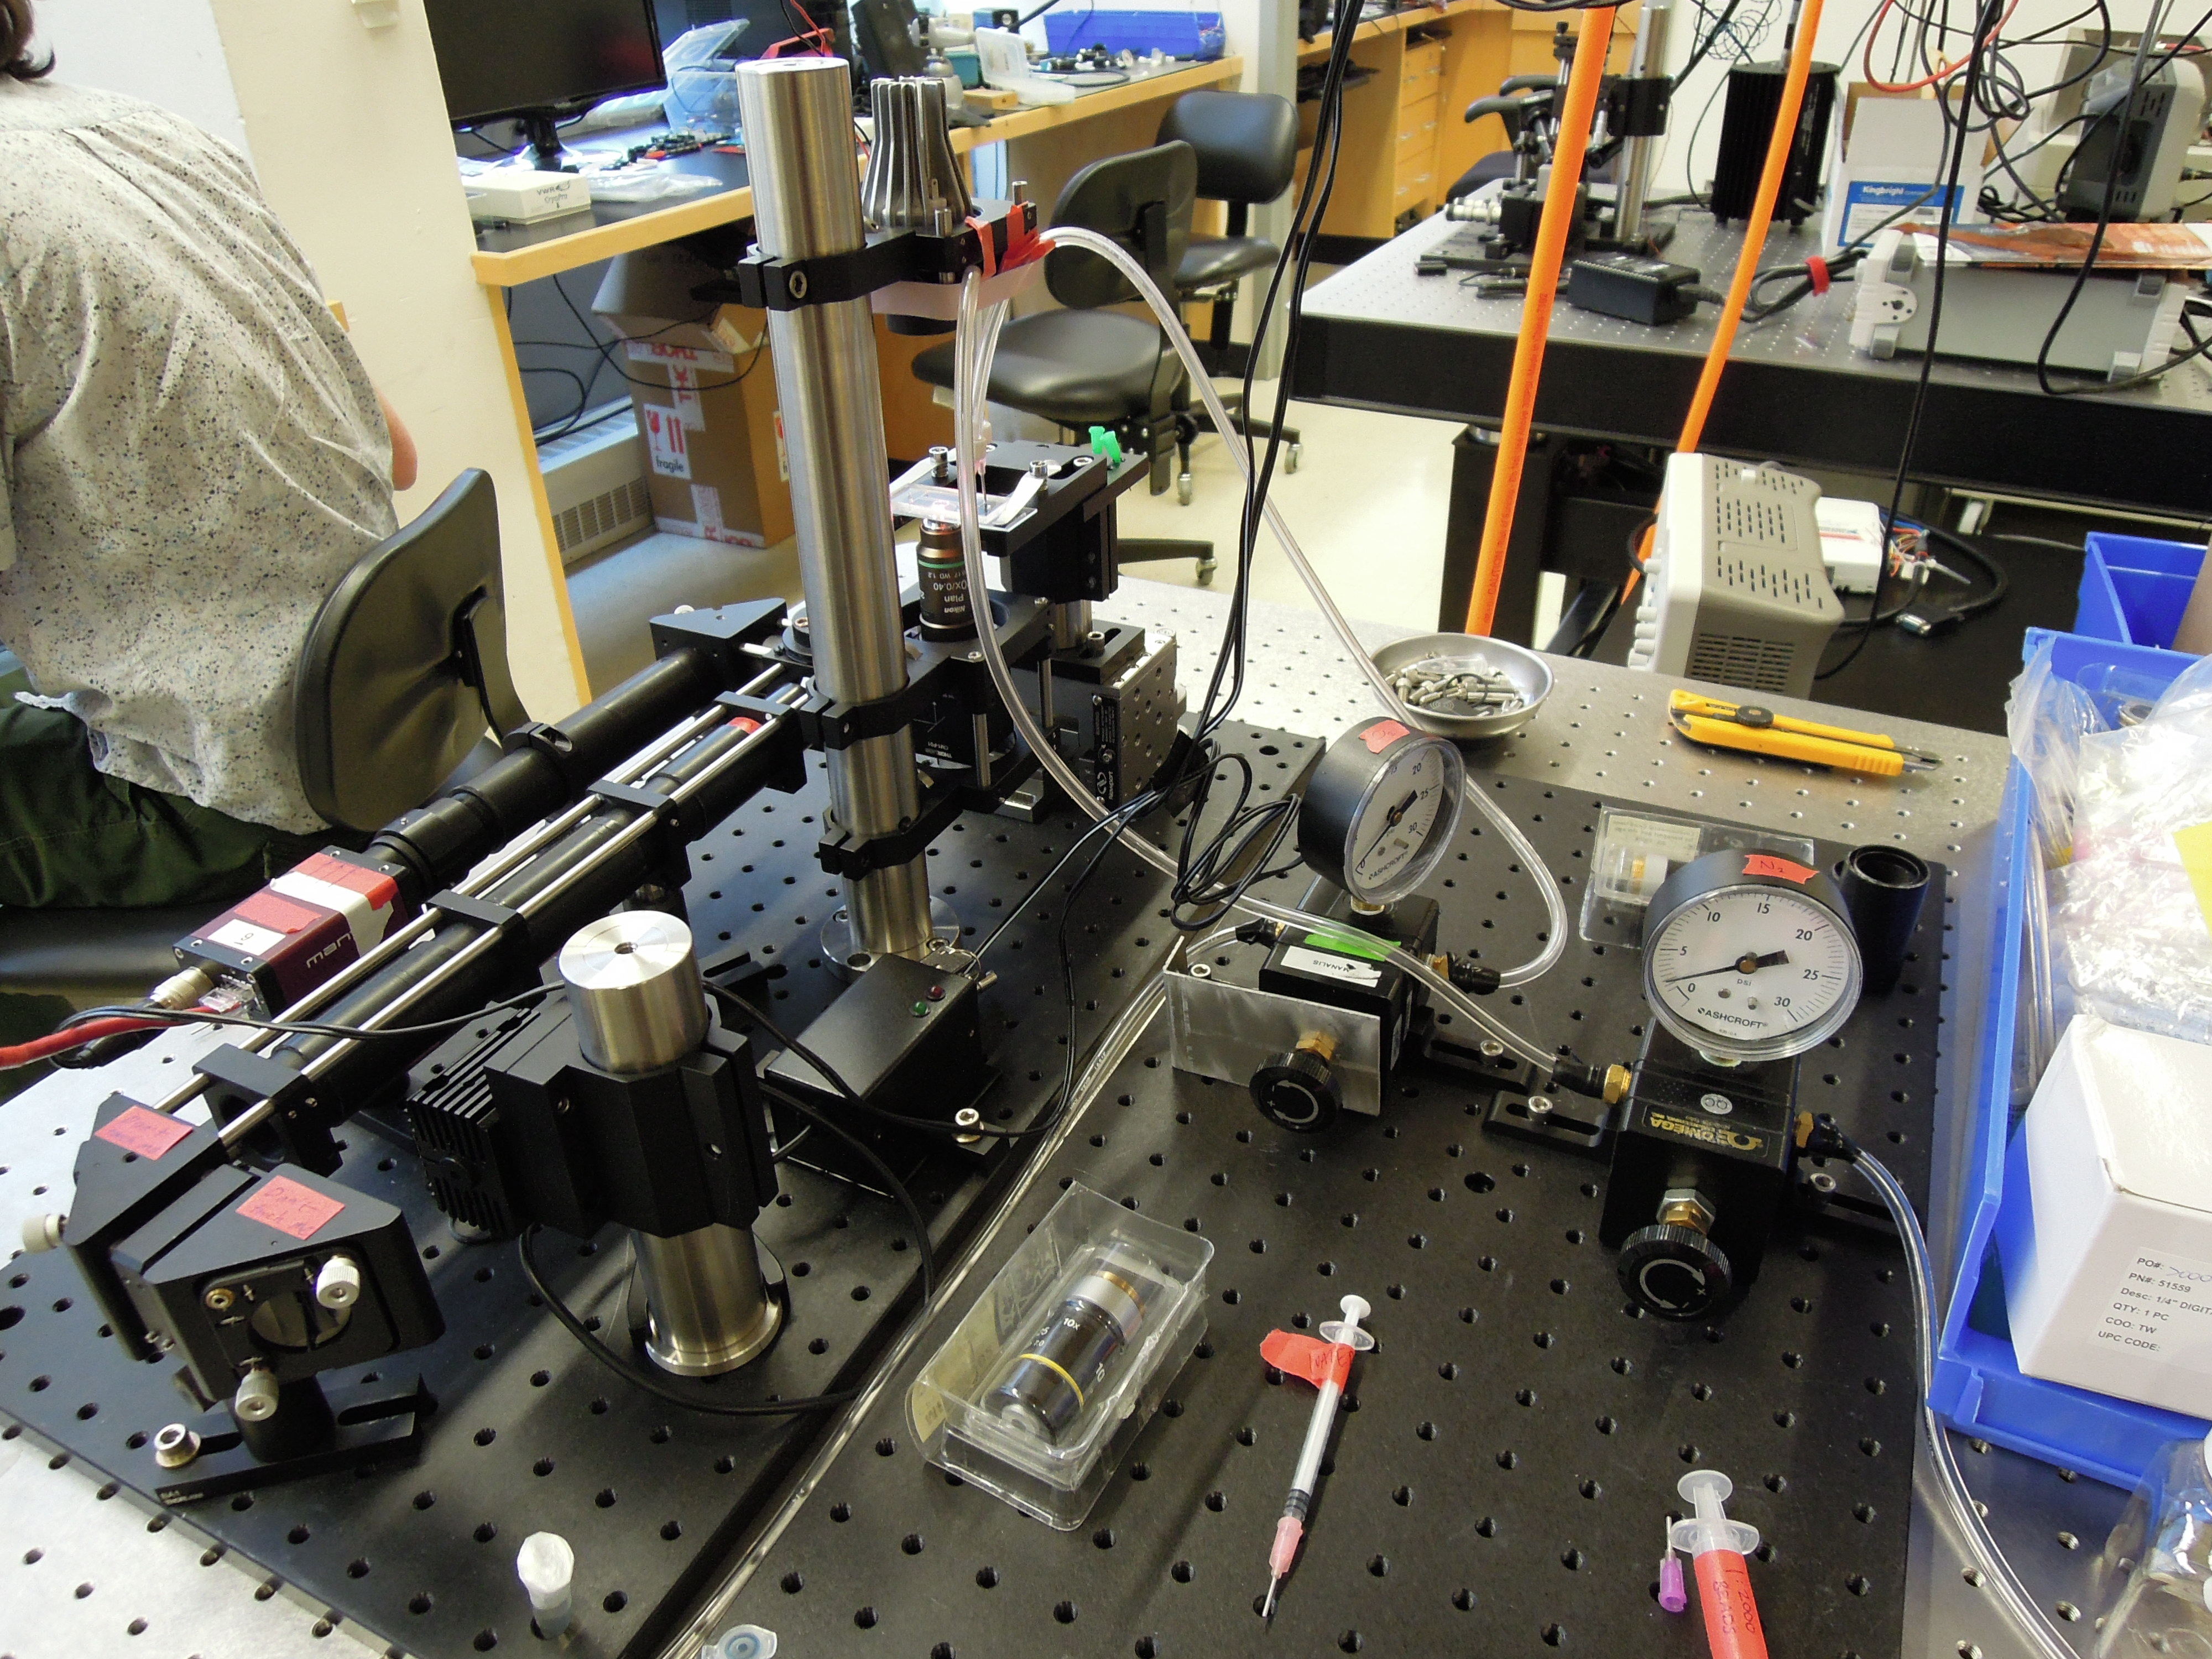
\includegraphics[width=\textwidth]{plots/Setup.jpg}
	\caption{The full experimental setup. The microfluidic device is on the stage of the microscope, which was custom-built for these experiments. The gas regulators allow for controlled flow of O\textsubscript{2} and N\textsubscript{2} gas into the device via syringe tips inserted into the device inlets.}
	\label{fig:SetupPhoto}
\end{figure}

\subsection{The microscope}

The microscope used for the project is a standard 4f microscope with 200mm Nikon objectives. The objective is mounted inverted to facilitate access to the sample. 10X and 20X objectives were used to collect micrographs during the course of the experiments. Brightfield illumination is provided by a red LED and collimated by a small lens. A barrier filter filters out other illumination from the CCD. These components are shown in  \Fref{fig:MicroscopeDiagram}.

A fluorescence pathway was also built to aid in cell tracking. The fluorescence illumination is provided by a 532 nm green laser source, which is expanded and then focused onto the surface of the objective in order to produce a collimated beam on the sample. A dichroic mirror reflects laser light onto the sample while allowing light emitted by fluorescence to pass through to the CCD.

Calibration was done optically using an Air Force Microscope Target and an image capture program to verify the magnification. By measuring the pixels in a photograph of a known distance, and knowing the dimensions of the imager in the CCD, the magnification can be calculated.

\begin{figure} 
	\centering
    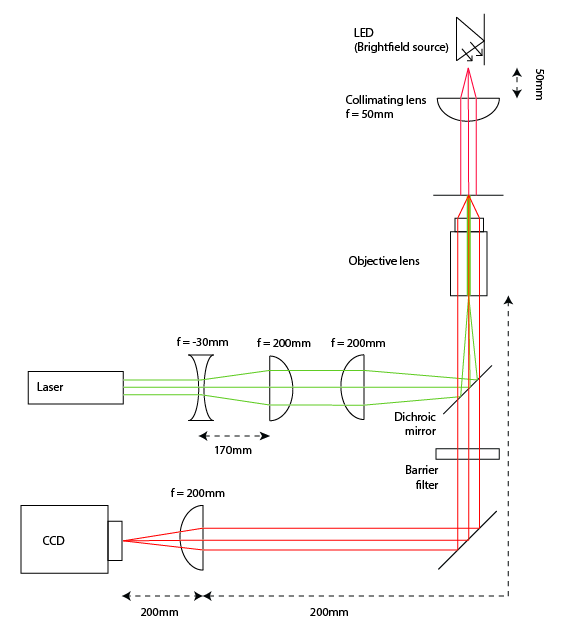
\includegraphics[width=\textwidth]{plots/MicroscopeDiagram.png}
	\caption{The fluorescence path (green), brightfield light source, and imaging path (red) of the microscope used to capture data from the microfluidic device with a CCD camera.}
	\label{fig:MicroscopeDiagram}
\end{figure}

\subsection{The microfluidic device} % Logan or Kiarash?

The microfluidic device is composed of the elastomeric material Polydimethylsiloxane (PDMS). The mask, a silicon wafer obtained from the MIT Environmental Microfluidics Group, was used in conjunction with UV-curing photopolymers to create a master mold for the PDMS devices. PDMS and its curing agent were mixed in a 10:1 ratio, respectively, and poured over the mold in a dish. The dish was degassed in a vacuum chamber and then cured for approximately 12 hours. After the PDMS had cured, the excess around the device was cut away, yielding the rectangular shape shown in \Fref{DevicePhoto}, and 0.050'' holes were punched through the device to allow access to the ends of each channel. After the device was completed, one side was treated with oxygen plasma, and it was bonded to a glass slide.

The device has three parallel channels formed by indentations in the PDMS; the glass slide creates the fourth wall of each channel, closing them. Each channel is 600 microns wide and 50 microns deep, with 200 microns of separation between each channel. Bacteria was injected into the center channel and allowed to settle before data collection began. Oxygen and nitrogen flows were directed down the outside channels. The devices were cleaned with isopropanol, which does not degrade the PDMS or the plasma bond, and reused for multiple experiments.

\begin{figure} 
	\centering
    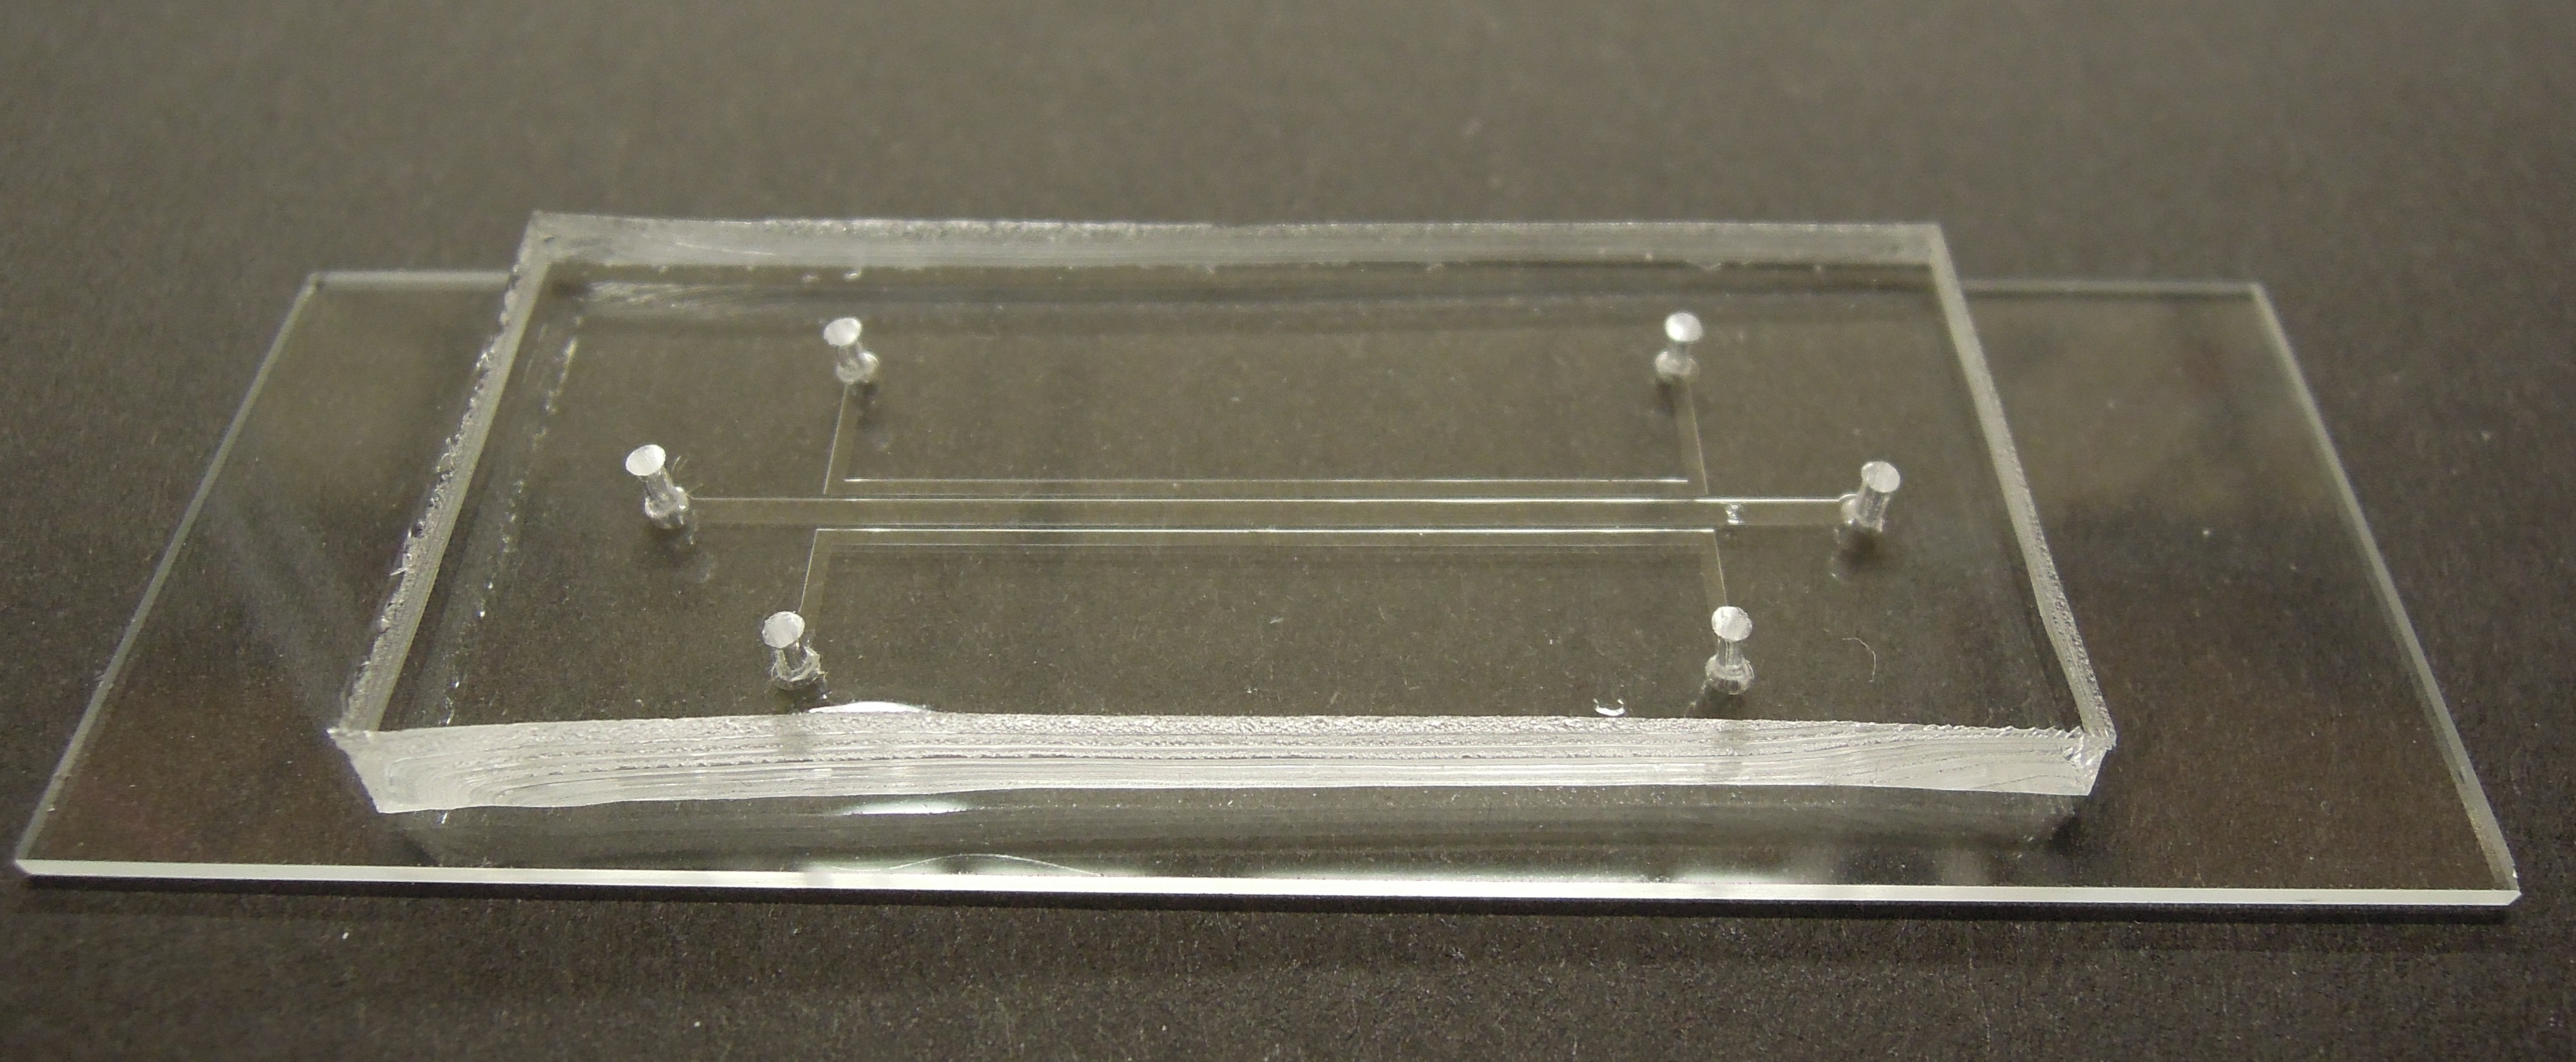
\includegraphics[width=\textwidth]{plots/Device.jpg}
	\caption{The microfluidic device. It is composed of PDMS, a silicone-like polymer, and features 3 channels parallel to each other. The center is wider and holds the bacteria, while the other two are thinner and flow gas through them. PDMS is gas-permeable, so the gas will diffuse into the center channel where the bacteria are located.}
	\label{fig:DevicePhoto}
\end{figure}

\subsection{Gas flow} % Kat?

The essence of aerotaxis is the gas gradient to which bacteria respond. The gas gradient was achieved by routing oxygen and nitrogen through the outside microfluidic channels parallel to the bacteria chamber. Both gases originate in storage cylinders attached to primary regulators. These regulators drop the gas pressure from about 2000 psi to 25 psi. After exiting the primary regulator, each gas flows through 1/8" ID Tygon E-3603 tubing to a secondary regulator that drops the pressure further, providing 2 psi to the lines connected to the device.

These lines have two different configurations during the experiment, providing either N\textsubscript{2} to one microfluidic gas channel and O\textsubscript{2} to the other, or providing N\textsubscript{2} to both microfluidic gas channels. These configurations are shown in \Fref{GasFlow} as a switch. Two lines of tubing interface with the device via Luer lock fittings attached to 0.050'' OD syringe tips that mate with 0.050'' ID access holes in the PDMS. One of these two lines is permanently connected to the nitrogen flow through a T-junction. The other line switches between the T-junction and the secondary O\textsubscript{2} regulator, depending on the experiment phase.  The gases flow through the device, diffusing into the PDMS to reach the bacteria chamber, and ultimately exhaust to the environment through the access holes at the channels� other ends.

\begin{figure} 
	\centering
    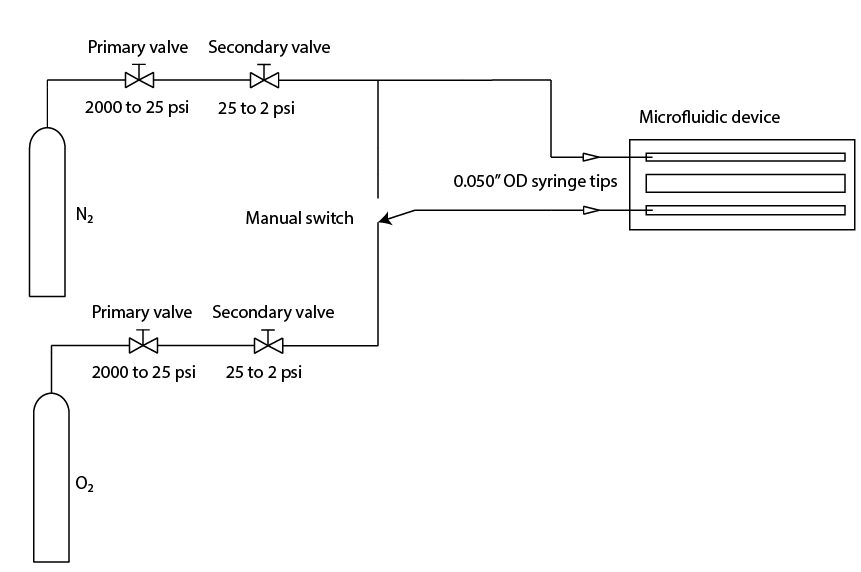
\includegraphics[width=\textwidth]{plots/GasFlow.png}
	\caption{The gas flow path, from the cylinders to the microfluidic device, which ultimately exhausts to air. The gas lines switch, providing N2 to one microfluidic gas channel and either N2 or O2 to the other gas channel, depending on the experiment phase.}
	\label{fig:GasFlow}
\end{figure}

\subsection{Bacteria culturing} % Brian?
\section{Results} % all of us

\begin{figure}[h!] 
  \centering
    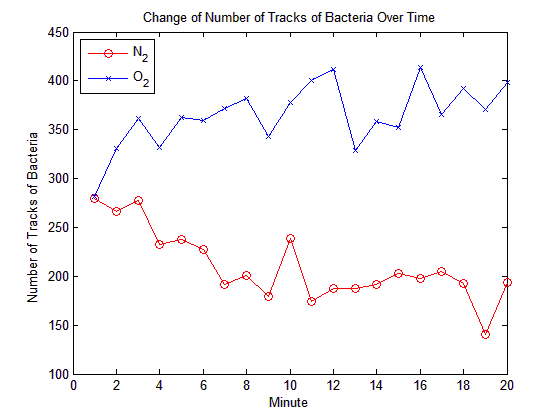
\includegraphics[width=\textwidth]{plots/number_Tracks.png}
      \caption[Number of trackable bacteria]{The number of trackable bacteria adjacent on the nitrogen side of the channel as compared to the number on the oxygen side. \\
      
      This plot was produced by finding bright centroids in captured microscope frames, and tracking the motion of the centroids. The number of ``tracks'' produced corresponds to the number of trackable bacteria.}
\end{figure}

\begin{figure}[h!] 
  \centering
    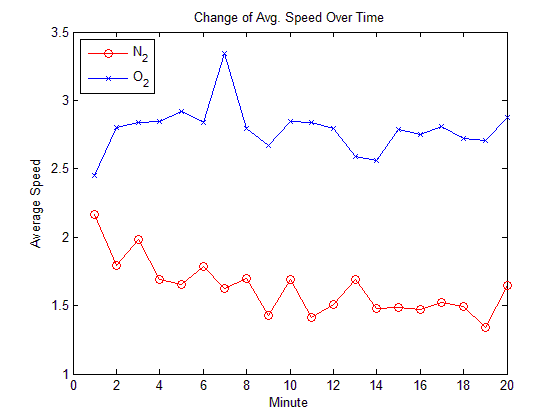
\includegraphics[width=\textwidth]{plots/average_speed.png}
      \caption[Number of trackable bacteria]{The number of trackable bacteria adjacent on the nitrogen side of the channel as compared to the number on the oxygen side. \\
      
      This plot was produced by finding bright centroids in captured microscope frames, and tracking the motion of the centroids. The number of ``tracks'' produced corresponds to the number of trackable bacteria.}
\end{figure}

\begin{figure}[h!] 
  \centering
    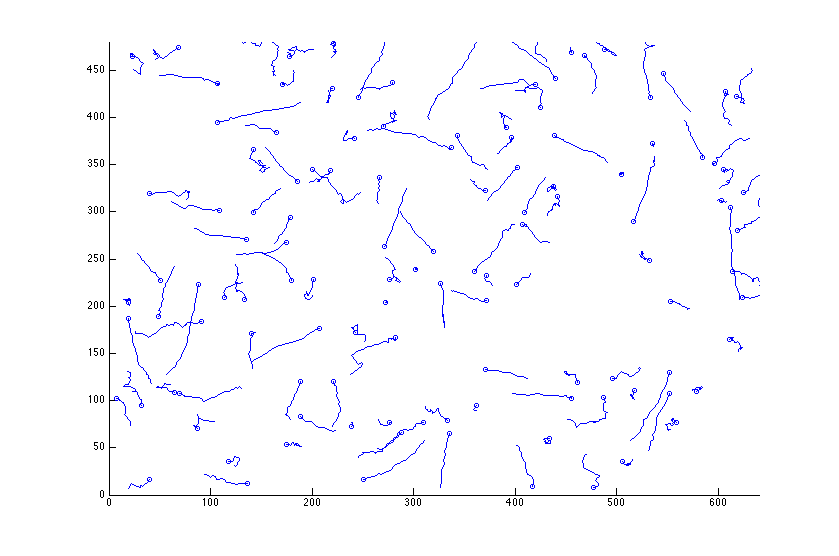
\includegraphics[width=0.5\textwidth]{plots/tracks_1.png}
    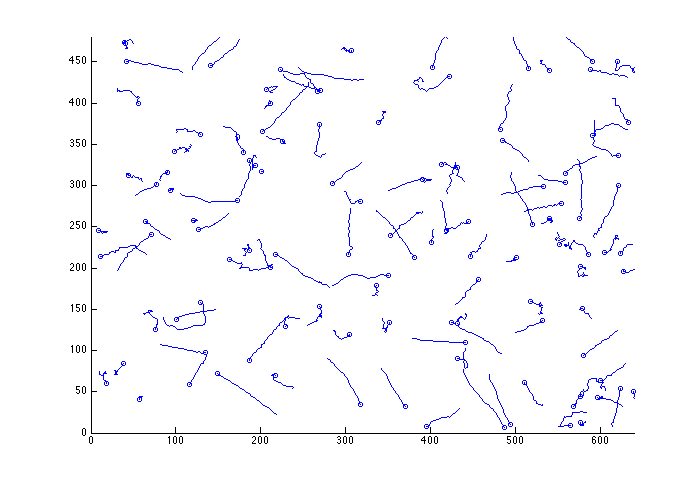
\includegraphics[width=0.5\textwidth]{plots/tracks_2.png}
    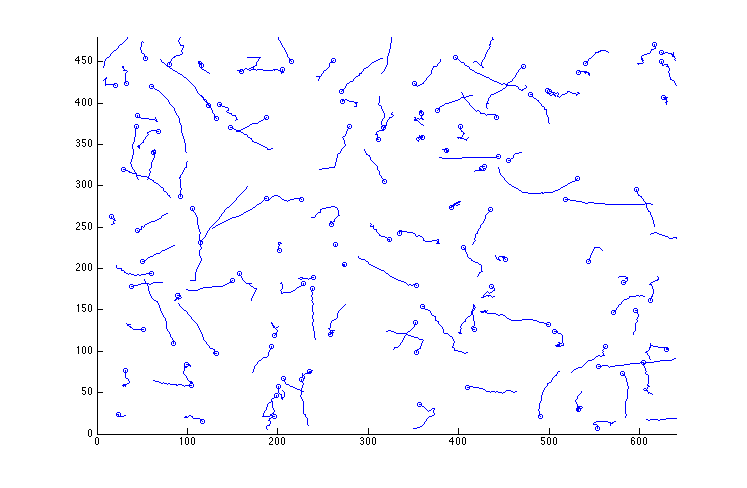
\includegraphics[width=0.5\textwidth]{plots/tracks_3.png}
      \caption[Representative traces]{Representative traces of bacteria motion. \\
      
      These plots were produced by finding bright centroids in captured microscope frames, and then finding centroids in sequential frames that are likely to belong to the same bacteria. These are plotted prior to gas flow switch, just after gas flow switch, and several minutes after gas flow switch, though no difference is apparent visually.}
\end{figure}

\begin{figure}[h!] 
  \centering
    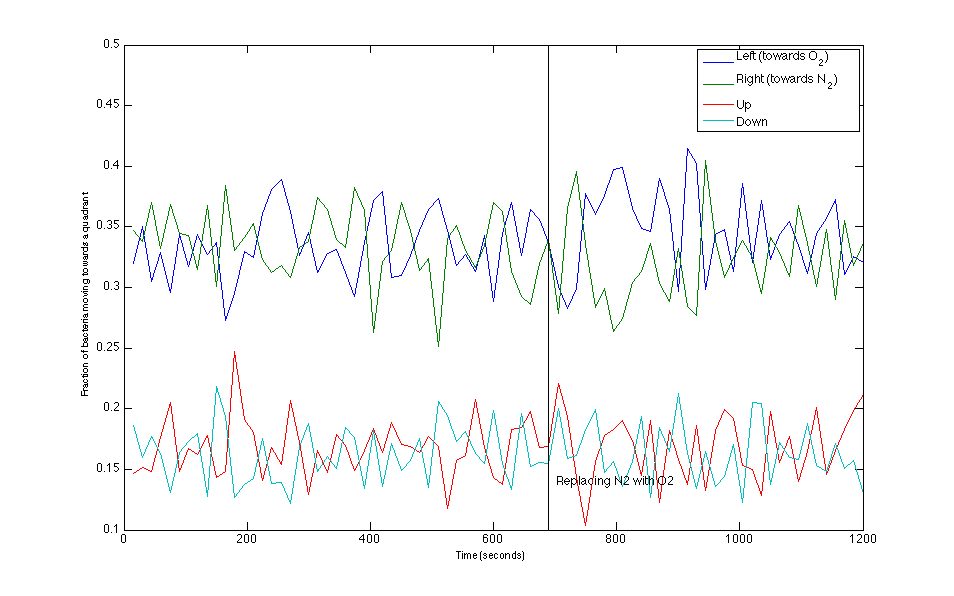
\includegraphics[width=\textwidth]{plots/direction.png}
      \caption[Bacterial motion]{Motion of motile bacteria divided into four quadrants, left (towards oxygen), right (towards nitrogen, up, and down.) This shows data from one representative experiment. \\
      
      This graph was produced by calculating the distance traveled and direction of travel for every bacteria ``track'' in each sequence of 30 frames. Bacteria that moved a significant amount were considered ``motile,'' all other bacteria were discarded. The bacteria were divided by dividing their motion into the four previously mentioned quadrants.}
\end{figure}

\begin{figure}[h!] 
  \centering
    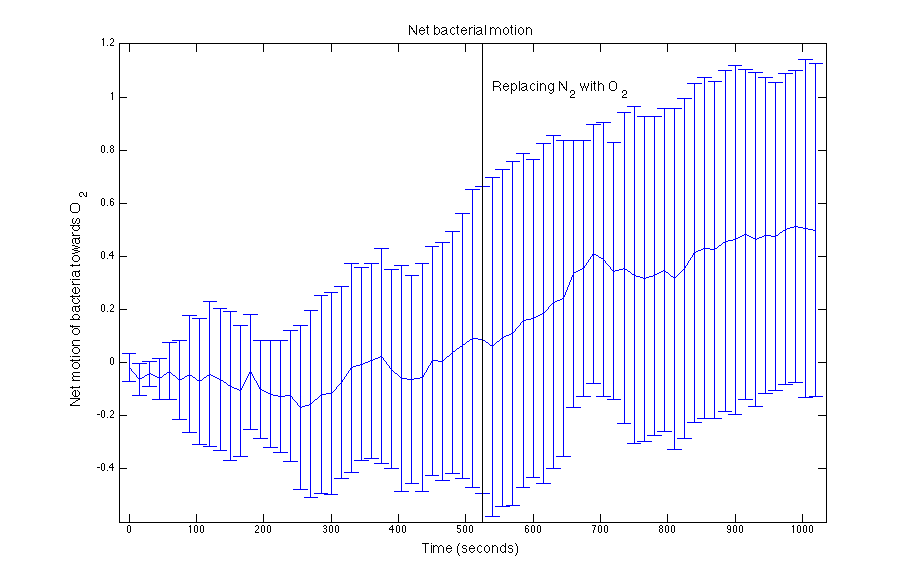
\includegraphics[width=\textwidth]{plots/cum_motion.png}
	\caption[Cumulative motion]{The cumulative percentage of net bacterial movement towards the oxygen side of the channel, averaged over 5 experimental trials. The x-axis is scaled relative to the number of visible bacteria in a single frame. \\
      
      This plot was produced by taking the cumulative sum of the difference between the ``left'' and ``right'' quadrants in the preceding figure. This sum is averaged over five trials. Error bars represent the standard deviation of that cumulative sum over the five trials (they grow with time because error is also being integrated in the cumulative sum). The size of the error bars is caused by a small $n$ (5), and integrated error. \\
      
      Note that there appears to be some drift prior to the gas line switch. This is likely due to random motion of the bacteria, and the large uncertainty in the data.}
      
\end{figure}


\section{Discussion} % all of us

\begin{thebibliography}{9}

\bibitem{15years} Taylor, B.L, Igor B. Zhulin, and Mark S. Johnson. ''Aerotaxis and other energy-sensing behavior in bacteria.'' Annu Rev Microbiol. 1999;53:103-28.
\bibitem{modelI} Tindall, M.K., P.K. Maini, S.L. Porter, and J.P. Armitage. ''Overview of Mathematical Approaches Used to Model Bacterial Chemotaxis I: The Single Cell.'' Bull Math Biol. 2008 Aug;70(6):1525-69. doi: 10.1007/s11538-008-9321-6. Epub 2008 Jul 19.
\bibitem{modelII} Tindall, M.K., P.K. Maini, S.L. Porter, and J.P. Armitage. ''Overview of Mathematical Approaches Used to Model Bacterial Chemotaxis II: Bacterial Populations.'' Bull Math Biol. 2008 Aug;70(6):1570-607. doi: 10.1007/s11538-008-9322-5. Epub 2008 Jul 19.

\end{thebibliography}

\end{document}  